%!TeX root=../tese.tex
%("dica" para o editor de texto: este arquivo é parte de um documento maior)
% para saber mais: https://tex.stackexchange.com/q/78101

\chapter{Algoritmo para MSF decremental}

\enlargethispage{.8\baselineskip}

Neste capítulo, estudaremos o problema da árvore geradora mínima em grafos dinâmicos. 
Dado um grafo conexo $G$ com um custo associado a cada uma de suas arestas, 
o problema da árvore geradora mínima consiste em determinar uma árvore geradora
de G com custo mínimo, onde o custo de uma árvore é a soma dos custos de suas arestas. 
Como estamos interessados em grafos dinâmicos, é natural remover a restrição de que o 
grafo seja conexo, e neste caso considerar florestas geradoras maximais de custo mínimo 
(MSF, do inglês \emph{minimum spanning forest}). Chamamos um grafo com um custo 
associado a cada aresta de \textbf{grafo ponderado}. 

O problema da árvore geradora mínima em grafos ponderados (conexos) estáticos pode ser 
resolvido eficientemente, por exemplo, pelos algoritmos de Kruskal e de Prim. O algoritmo de Kruskal 
utiliza uma estrutura de dados clássica conhecida como union-find, enquanto que o algoritmo
de Prim utiliza uma fila de prioridades. Não há na literatura uma versão destes algoritmos 
para grafos dinâmicos. Isso talvez se deva à característica essencialmente sequencial destes
algoritmos, que modificam suas estruturas internas conduzidos por uma ordem de eventos.
Uma alteração no grafo poderia levar a uma alteração em toda a sequência de eventos 
nesses algoritmos a partir de um certo ponto, e com isso não há uma versão eficiente deles
que acomode alterações no grafo. 

Por outro lado, Holm, de Lichtenberg e Thorup~\cite{jacob_holm} propuseram uma adaptação do seu algoritmo para conexidade em 
grafos dinâmicos, apresentado no Capítulo 2, para que este mantenha, de maneira eficiente, 
uma floresta geradora maximal de custo mínimo em um grafo ponderado que pode sofrer 
remoções de arestas.  Ou seja, eles propuseram um algoritmo que resolve de maneira 
eficiente o problema que chamamos de MSF decremental.  Neste capítulo, descreveremos
esse algoritmo, que é uma adaptação do algoritmo descrito no Capítulo 2 para que este 
passe a resolver o problema da MSF decremental.  

\section{Biblioteca da MSF decremental}
\label{sec:decremental-msf-library}

Implementar o algoritmo decremental para florestas geradoras maximais de custo mínimo (MSF, de \textit{Minimum Spanning Forest}) resume-se à construção da seguinte biblioteca de forma eficiente:

\begin{itemize}
    \item \texttt{\textbf{MSFDecremental(n, E)}}: contrói e devolve um grafo ponderado $G$ com $n$ vértices e as arestas $E$;
    \item \texttt{\textbf{conectadosMSF(G, u, v)}}: devolve verdadeiro se os vértices $u$ e $v$ estão na mesma componente de $G$ e falso caso contrário;
    \item \texttt{\textbf{removaMSF(G, u, v)}}: remove a aresta $uv$ do grafo $G$.
\end{itemize} 

Note que, diferente da biblioteca do algoritmo de conexidade em grafos dinâmicos, apresentada na Seção~\ref{sec:dynamic-graph-routines}, na MSF decremental não temos um método equivalente a \texttt{adicioneGD} disponível para o usuário. Em nossa implementação \cite{chung2025}, para criarmos um grafo $G$ de $n$ vértices e $m$ arestas ponderadas dadas no conjunto $E$, chamamos \texttt{MSFDecremental($n$, $E$)}, onde criamos $\left\lceil \lg n \right\rceil$ florestas e $\left\lceil \lg n \right\rceil$ listas de adjacências com $n$ vértices isolados. Em seguida, ordenamos e inserimos essas $m$ arestas em ordem crescente de peso, usando uma biblioteca pronta do $\emph{C++}$ para ordená-las, que consome tempo esperado $\Oh(n \lg n)$. Estas $m$ arestas são  inseridas uma a uma acionando \texttt{adicioneMSF(u, v, p)}, onde $u$ e $v$ são pontas da aresta e $p$ é o peso dela.

A rotina \texttt{adicioneMSF} é acionada somente dentro do construtor. Por ser uma rotina privada, ou seja, não está disponível para o usuário, após a inserção destas arestas, não é permitido mais operações de inserção, somente de remoção de arestas. Para o usuário, então, só estarão disponíveis as rotinas \texttt{conectadosMSF} e \texttt{removaMSF} como consultas ao grafo. A versão totalmente dinâmica, que inclui a rotina \texttt{adicioneMSF} para o usuário, será estudada posteriormente na Seção~\ref{sec:fully-MSF}.

O construtor \texttt{MSFDecremental}, devido à ordenação de arestas, possui consumo de tempo $\Oh(n \lg n)$. Já a rotina \texttt{conectadosMSF} possui consumo de tempo amortizado $\Oh(\lg n)$, a mesma do \texttt{conectadosGD}. Como estes dois métodos são muito parecidos com os do algoritmo de conexidade em grafos dinâmicos, passaremos brevemente sobre eles, e detalharemos mais a rotina \texttt{removaMSF}, que possui a rotina auxiliar \texttt{substituaArestaMSF} implementada de maneira diferente do \texttt{substituaAresta} do algoritmo de conexidade em grafos dinâmicos. 

Usaremos várias definições já apresentadas no algoritmo do grafo dinâmico, incluindo as mesmas invariantes apresentadas na Seção~\ref{sec:level-slicing}, os mesmos tipos de arestas da Seção~\ref{sec:dynamic-graph-edge-types} e nós das florestas apresentados na Seção~\ref{sec:graph-nodes}. A seguir, apresentaremos as rotinas da MSF decremental e alguns ajustes a serem feitos. 

\subsection{Listas de adjacências}
\label{sec:adjancency-lists-min-heap}

Na Seção~\ref{sec:dynamic-graph-edge-types}, apresentamos a biblioteca de \texttt{listasDeAdjacências}, onde usamos um mapa hash para inserir ou remover um vértice $v$ da lista de $u$, além de percorrer os vizinhos da lista de $u$. No algoritmo da MSF decremental, quando removemos uma aresta de nível $i$ da floresta $F_i$, uma componente desta será quebrada em duas, $T_u$ e $T_v$, da mesma forma que no algoritmo de conexidade em grafos dinâmicos. A diferença é que, no caso da MSF decremental, precisamos buscar por uma aresta substituta que tenha o menor peso e que ligue $T_u$ a~$T_v$. Não podemos simplesmente percorrer todos os vizinhos $v$ de cada vértice $u$ em $T_u$, verificar se $uv$ reconecta as componentes separadas e se é de menor peso dentre todas as substitutas, já que isso seria ineficiente.

Assim, fica claro que seria bom percorrer as arestas reservas em ordem crescente de peso e testar se alguma é substituta nesta ordem. Por isso, em vez de usar um mapa hash para mapear os vizinhos das listas de adjacências de cada vértice, usaremos um min-heap. Na verdade, como estamos trabalhando com nós de vértice e de aresta, cada nó de vértice $u$ guardará um min-heap com os vizinhos de $u$, onde a chave dessa estrutura de dados para um vizinho $v$ será o peso da aresta $uv$. Nós de aresta também guardarão um min-heap, porém vazio. 

A biblioteca do min-heap está descrita a seguir.

\begin{itemize}
    \item \texttt{\textbf{MinHeap(u)}}: cria um min-heap vazio para o vértice $u$ (em nossa implementação, criamos um vetor vazio);
    \item \texttt{\textbf{éVazio(MH, u)}}: devolve verdadeiro se o min-heap MH de $u$ está vazio e falso caso contrário;
    \item \texttt{\textbf{tamanho(MH, u)}}: retorna a quantidade de vizinhos no min-heap MH de $u$;
    \item \texttt{\textbf{remova(MH, u, v)}}: remove o vizinho $v$ do min-heap MH de $u$;
    \item \texttt{\textbf{consulteMínimo(MH, u)}}: retorna um par $\{v, p\}$ do min-heap MH de $u$, onde $v$ é um vizinho de $u$ com chave mínima $p$;
    \item \texttt{\textbf{extraiaMínimo(MH, u)}}: remove o par $\{v, p\}$ do min-heap MH de $u$, onde $v$ é o vizinho de $u$ com chave mínima $p$;
    \item \texttt{\textbf{insira(MH, u, v, p)}}: insere o vizinho $v$ no min-heap MH de $u$, onde $p$ é sua chave, ou seja, é o peso da aresta $uv$.
\end{itemize} 

Os métodos \texttt{remova}, \texttt{extraiaMínimo} e \texttt{insira} consomem tempo O($\lg n)$ usando uma implementação tradicional de heap sort de Thomas H. Cormen et al. \cite{clrs}. O resto dos métodos consomem tempo constante, e eles serão necessários para buscar a aresta substituta de peso mínimo, como descreveremos mais à frente.

Com base na biblioteca do min-heap, podemos definir a biblioteca das listas de adjacências da MSF decremental. 

\begin{itemize}
    \item \texttt{\textbf{listasDeAdjacênciasMSF(n)}}: constrói e devolve um grafo com $n$ vértices e sem arestas, representado por listas de adjacências;
    \item \texttt{\textbf{adicioneLAMSF(R, u, v, p)}}: adiciona o vértice $u$ na lista de adjacências de $v$ em $R$ e vice-versa, considerando que o peso de $uv$ é $p$;
    \item \texttt{\textbf{removaLAMSF(R, u, v)}}: remove o vértice $u$ da lista de adjacências de $v$ em $R$ e vice-versa.
\end{itemize} 

Uma chamada à rotina \texttt{adicioneLAMSF(R, u, v, p)} aciona \texttt{insira(MH, u, v, p)} e \texttt{insira(MH, v, u, p)}, consumindo tempo $\Oh(\lg n)$. Similarmente, uma chamada à rotina \texttt{removaLAMSF(R, u, v)} aciona \texttt{remova(MH, u, v)} e \texttt{remova(MH, v, u)}, consumindo também tempo $\Oh(\lg n)$.

Como o min-heap é uma estrutura de dados bastante conhecida, não iremos descrever a sua implementação em detalhes. O objetivo é ressaltar as diferenças entre as listas de adjacências utilizadas no algoritmo de conexidade em grafos dinâmicos e na MSF decremental, e como essa mudança afetará o comportamento do método \texttt{substituaArestaMSF} da MSF decremental.

\section{Rotinas da biblioteca da MSF decremental}

\subsection{Criação do grafo}

A rotina \texttt{MSFDecremental}, como se pode ver no Programa~\ref{prog:newDecrementalMSF}, é bem parecida com a do grafo dinâmico, descrita na Seção~\ref{sec:dynamic-graph-creation}. 

\begin{programruledcaption}{\texttt{MSFDecremental($n$, $E$)} \label{prog:newDecrementalMSF}}
    \noindent\textbf{Entrada}: Recebe o número $n$ de vértices do grafo e um conjunto de arestas $E$. \\
    \textbf{Saída}: Devolve um grafo $G$ com $n$ vértices e $m$ arestas ponderadas.
    \vspace{-0.5\baselineskip}
    \begin{lstlisting}[
        language={[brazilian]pseudocode},
        style=pseudocode,
        style=wider,
        functions={},
        specialidentifiers={},
        escapeinside={(*@}{@*)},
    ]
    L := $\left\lceil \lg n \right\rceil$
    $\dotvar{G}{nívelMax}$ := L
    \textbf{para} $i$ := $1$ \textbf{até} $L$ \textbf{faça}
        $G.F_i$ := \texttt{florestaDinâmica($n$)}
        $G.R_i$ := \texttt{listasDeAdjacênciasMinHeap($n$)}
    $\dotvar{G}{nível}$ := \texttt{novoMapaHash($n$)}
    \texttt{ordene($E$)} (*@\hfill $\triangleright$ ordena as arestas do conjunto $E$ em ordem crescente@*)
    \textbf{para cada aresta} ($u$, $v$, $p$) \textbf{em} $E$ \textbf{faça}
        \texttt{adicioneMSF}($G$, $u$, $v$, $p$)
    \textbf{retorne} G
    \end{lstlisting}
    \vspace{-0.5\baselineskip}
\end{programruledcaption}

Podemos notar algumas diferenças quando comparamos o construtor \texttt{MSFDecremental} com o \texttt{grafoDinâmico}. Na MSF decremental, além de inicializarmos $\left\lceil \lg n \right\rceil$ listas de adjacências e $\left\lceil \lg n \right\rceil$ florestas dinâmicas, ordenamos arestas do conjunto $E$ em ordem crescente e inserimos uma a uma chamando \texttt{adicioneMSF}, que está descrito abaixo.

\begin{programruledcaption}{\texttt{adicioneMSF($G$, $u$, $v$, $p$)} \label{prog:addMSF}}
    \noindent\textbf{Entrada}: Recebe dois vértices $u$ e $v$ do grafo $G$, com $u < v$, e o peso $p$ da aresta $uv$. \\
    \textbf{Efeito}: Adiciona a aresta $uv$ de peso $p$ no grafo $G$.
    \vspace{-0.5\baselineskip}
    \begin{lstlisting}[
        language={[brazilian]pseudocode},
        style=pseudocode,
        style=wider,
        functions={},
        specialidentifiers={},
        escapeinside={(*@}{@*)},
    ]
    L := $\dotvar{G}{nívelMax}$
    $\dotvarm{G}{nível}{u,v}$ := $L$
    \textbf{se} \texttt{conectadosFD($G.F_{L}$, $u$, $v$)} \textbf{então} (*@\hfill $\triangleright$ $uv$ é aresta reserva@*)
        \texttt{adicioneLAMSF($G.R_{L}$, $u$, $v$, $p$)}
        \texttt{incrementeArestasReservasDeNível($G.F_{L}$, $G.R_{L}$, $u$)}
        \texttt{incrementeArestasReservasDeNível($G.F_{L}$, $G.R_{L}$, $v$)}
    \textbf{senão}
        \texttt{adicioneFD($G.F_L$, $u$, $v$, $p$)}
        \texttt{atualizeÉNível($G.F_L$, $u$, $v$, $\textbf{verdadeiro}$)}
    \end{lstlisting}
    \vspace{-0.5\baselineskip}
\end{programruledcaption}

Como citada antes, a rotina \texttt{adicioneMSF} é acionada exclusivamente em \texttt{MSFDecremental}. Ademais, a única diferença entre a \texttt{adicioneMSF} e a \texttt{adicioneGD} que vimos é que, na primeira, estamos guardando o peso das arestas quando as inserimos no grafo. Portanto, \texttt{adicioneMSF} também consome tempo amortizado $\Oh(\lg n)$ e as três invariantes são preservadas ao acionar \texttt{adicioneMSF}, já que estamos sempre inserindo arestas com nível $\left\lceil \lg n \right\rceil$ em $F_L$ e as florestas de níveis inferiores não são afetadas com a inserção.

\subsection{Consultas de conexidade na MSF decremental}
\label{sec:connectivity-test-MSF}

A rotina \texttt{conectadosMSF}, descrita abaixo, é igual a \texttt{conectadosGD}. Mudamos apenas o seu nome para ficar coerente com os nomes dos métodos da biblioteca da MSF decremental. 

\begin{programruledcaption}{\texttt{conectadosMSF($G$, $u$, $v$)} \label{prog:connectedMSF}}
    \noindent\textbf{Entrada}: Recebe dois vértices $u$ e $v$ do grafo $G$. \\
    \textbf{Saída}: Devolve um booleano indicando se $u$ e $v$ estão conectados em $G$.
    \vspace{-0.5\baselineskip}
    \begin{lstlisting}[
        language={[brazilian]pseudocode},
        style=pseudocode,
        style=wider,
        functions={},
        specialidentifiers={},
        escapeinside={(*@}{@*)},
    ]
    L := $\dotvar{G}{nívelMax}$
    retorne \texttt{conectadosFD($G.F_L$, $u$, $v$)}
    \end{lstlisting}
    \vspace{-0.5\baselineskip}
\end{programruledcaption}

\raggedbottom

Da mesma forma que em \texttt{conectadosGD}, a rotina \texttt{conectadosMSF} também consome tempo amortizado $\Oh(\lg n)$. Além disso, a rotina de consulta não altera o nosso grafo, incluindo florestas e listas de adjacências, já que não há nenhuma modificação neles. Isso implica que as três invariantes são mantidas. 

\subsection{Remoção de arestas na MSF decremental}
\label{sec:decremental-MSF-edge-removal}

A remoção de arestas também é semelhante à do algoritmo de conexidade em grafos dinâmicos. A diferença é que a busca por alguma aresta substituta, feita na \texttt{substituaArestaMSF} agora, é dada por ordem crescente de peso das arestas reserva. Quando removemos uma aresta $uv$ de nível $i$ em $F_i$, procuramos por alguma reserva de peso mínimo global dentre todas as reserva dm $R_i$, e testamos se ela é uma substituta. Se não, a rebaixamos para $R_{i-1}$ e buscamos a próxima de peso mínimo global em $R_i$. Assim, quando achamos uma substituta, conseguimos manter o peso da MST do grafo e ainda reconectar as duas componentes separadas devido à remoção de $uv$. 

O método \texttt{removaMSF} está descrito abaixo. Como se pode ver, não há alterações em sua estrutura além da mudança de nomes de alguns métodos.

\begin{programruledcaption}{\texttt{removaMSF($G$, $u$, $v$)} \label{prog:removeGD-version-msf}}
    \noindent\textbf{Entrada}: Recebe dois vértices adjacentes $u$ e $v$ do grafo $G$. \\
    \noindent\textbf{Efeito}: Remove a aresta $uv$ do grafo $G$. 
    \vspace{-0.5\baselineskip}
    \begin{lstlisting}[
        language={[brazilian]pseudocode},
        style=pseudocode,
        style=wider,
        functions={},
        specialidentifiers={},
        escapeinside={(*@}{@*)},
    ]
    L := $\dotvar{G}{nívelMax}$
    i := $\dotvarm{G}{nível}{u,v}$
    $\dotvarm{G}{nível}{u,v}$ := \texttt{NIL} (*@\hfill $\triangleright$ marcamos $uv$ como removida@*)
    \textbf{se} uv $\in$ G.$F_{L}$ \textbf{então}  (*@\hfill $\triangleright$ $uv$ é aresta da floresta@*)
        \textbf{para} j := i \textbf{até} L \textbf{faça}
            \texttt{removaFD($G.F_j$, $u$, $v$)}
        \texttt{substituaArestaMSF($G$, $i$, $u$, $v$)}
    \textbf{senão} (*@\hfill $\triangleright$ $uv$ é aresta reserva@*)
        \texttt{removaLAMSF($G.R_i$, $u$, $v$)}
        \texttt{decrementeArestasReservasDeNível($G.F_i$, $G.R_i$, $u$)}
        \texttt{decrementeArestasReservasDeNível($G.F_i$, $G.R_i$, $v$)}
    \end{lstlisting}
    \vspace{-0.5\baselineskip}
\end{programruledcaption}

A seguir, demonstraremos a remoção de uma aresta $uv$ da floresta em uma série de imagens. Na Figura~\ref{fig:example-replacement-msf1}, temos um grafo $G$ de $n = 10$ vértices. Para facilitar, assumiremos que, até o momento, só houve inserções de arestas. 

\begin{figure}[H]
    \centering

    \noindent
    \begin{minipage}[c]{2cm}
        \raggedright
        Nível $4$
    \end{minipage}%
    \begin{minipage}[c]{0.8\textwidth}
        \centering
        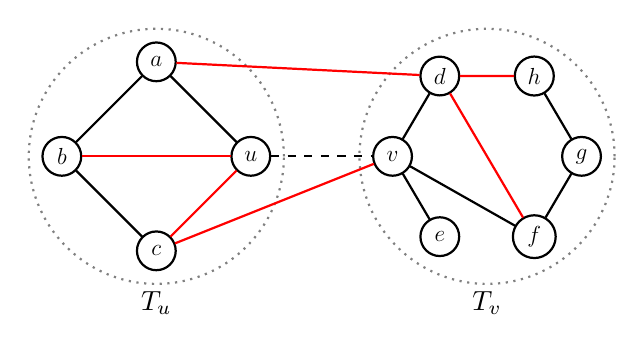
\begin{tikzpicture}
        [scale=0.6, node/.style={scale=0.7, circle,draw,minimum size=2em, thick, font=\large},
        edge/.style={thick, black},
        reserve/.style={red, thick},
        removed/.style={black, thick, dashed}]

        \node[node] (u) at (-1,2) {$u$};
        \node[node] (a) at (-3,4) {$a$};
        \node[node] (b) at (-5,2) {$b$};
        \node[node] (c) at (-3,0) {$c$};
        \node[node] (v) at (2,2) {$v$};
        \node[node] (d) at (3,3.7) {$d$};
        \node[node] (e) at (3,0.3) {$e$};
        \node[node] (f) at (5,0.3) {$f$};
        \node[node] (g) at (6, 2) {$g$};
        \node[node] (h) at (5, 3.7) {$h$};
        
         % Dotted circles for T_u and T_v
        \draw[dotted, thick, gray] (-3,2) circle (2.7cm);
        \draw[dotted, thick, gray] (4,2) circle (2.7cm);  
        
        % Labels for the circles
        \node at (-3,-1.1) {$T_u$};
        \node at (4,-1.1) {$T_v$};

        % tree edges (normal black edges)
        \draw[edge] (a) -- (u) node[midway, below] {};
        \draw[edge] (a) -- (b) node[midway, below] {};
        \draw[edge] (b) -- (c) node[midway, below] {};
        \draw[edge] (v) -- (d) node[midway, below] {};
        \draw[edge] (v) -- (f) node[midway, below] {};
        \draw[edge] (v) -- (e) node[midway, below] {};
        \draw[edge] (f) -- (g) node[midway, below] {};
        \draw[edge] (g) -- (h) node[midway, below] {};
        % reserve edges (normal red edges)
        
        \draw[removed] (u) -- (v) node[midway, below] {};
        \draw[reserve] (a) -- (d) node[midway, below] {};
        \draw[reserve] (c) -- (v) node[midway, below] {};
        \draw[reserve] (b) -- (u) node[midway, below] {};
        \draw[reserve] (c) -- (u) node[midway, below] {};
        \draw[reserve] (d) -- (f) node[midway, below] {};
        \draw[reserve] (d) -- (h) node[midway, below] {};

        \end{tikzpicture}
    \end{minipage}
    \vspace{1cm}
        \noindent
    \begin{minipage}[c]{2cm}
        \raggedright
        Nível $3$
    \end{minipage}%
    \begin{minipage}[c]{0.8\textwidth}
        \centering
        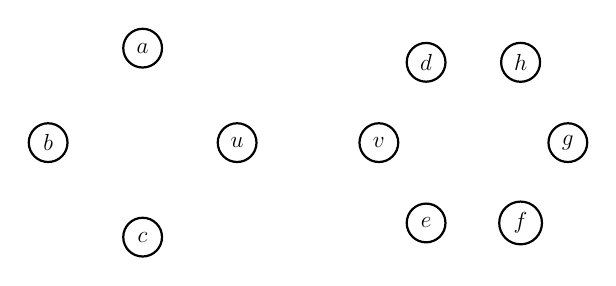
\begin{tikzpicture}
            [scale=0.6, node/.style={scale=0.7, circle,draw,minimum size=2em, thick, font=\large},
            edge/.style={thick, black},
            reserve/.style={red, thick},
            removed/.style={black, thick, dashed}]

            \node[node] (u) at (-1,2) {$u$};
            \node[node] (a) at (-3,4) {$a$};
            \node[node] (b) at (-5,2) {$b$};
            \node[node] (c) at (-3,0) {$c$};
            \node[node] (v) at (2,2) {$v$};
            \node[node] (d) at (3,3.7) {$d$};
            \node[node] (e) at (3,0.3) {$e$};
            \node[node] (f) at (5,0.3) {$f$};
            \node[node] (g) at (6, 2) {$g$};
            \node[node] (h) at (5, 3.7) {$h$};
            
            %\draw[edge] (a) -- (u) node[midway, below] {};
            %\draw[edge] (a) -- (b) node[midway, below] {};
            %\draw[edge] (b) -- (c) node[midway, below] {};

        \end{tikzpicture}
    \end{minipage}
    \caption{Um grafo $G$ de 10 vértices, onde as arestas pretas são da floresta $F_4$, enquanto as vermelhas são reservas. A aresta $uv$ está prestes a ser removida. A floresta $F_{4}$ de $G$ de cima contém todas as arestas pretas recém-inseridas e as arestas vermelhas estão em $R_4$. A floresta de baixo é a $F_{3}$, com os vértices isolados, e $R_3$ também não tem nenhuma aresta.}
    \vspace{-1cm}
    \label{fig:example-replacement-msf1}
\end{figure}
